\documentclass[compress,dvips,xcolor={dvipsnames},t]{beamer}

\usepackage[english]{babel}
\usepackage{graphicx}
\usepackage{amssymb,amsmath,amsthm}
\usepackage{xspace}

\newtheorem{proposition}{Proposition}
%\newtheorem{theorem}{Theorem}
\newcommand{\id}[1]{\textsf{#1}}
\newcommand{\coding}[4]{#1 \vdash #2 : #3 \rightarrow #4}
\newcommand{\decoding}[3]{{\cal D}(#1,#2,#3)}

\renewcommand{\refname}{}
\newcommand\ASN{\textsf{ASN.1}\xspace}
\newcommand{\core}{core \ASN}
\newcommand\Cpp{\mbox{\textsf{C} \hspace*{-2.5mm} \raise 0.7mm \hbox
{${\scriptscriptstyle \textsf{++}}$}}\xspace}

\title{Career overview}
\author{Christian Rinderknecht}
\date{10 March 2016}

\begin{document}

\frame{\maketitle}

\begin{frame}
  \frametitle{Career}

  Instead of a strict chronology, I propose a thematic approach:
  \begin{itemize}
    \item Compilation (front-ends, static analysis);
    \item Model-based testing (telecommunications);
    \item Didactics of formal languages (education).
  \end{itemize}

\end{frame}

\begin{frame}
\frametitle{Compiler Front-ends -- The case of \ASN}

The wide variety of hardware architectures and programming languages
calls for the definition of a universal format for data to be
exchanged over a computer network.

\medskip

\emph{Abstract Syntax Notation One} (\ASN) is a standardised language
(ISO, ITU-T) for defining data types whose values may be exchanged
across a network between two, possibly heterogeneous peers.

\medskip

\ASN is completed by a set of \emph{encodings} which serialise the
values into streams of bits, the two most prominent being
\begin{itemize}

  \item the Basic Encoding Rules (BER),

  \item and Packed Encoding Rules (PER).

\end{itemize}

\end{frame}

\begin{frame}
\frametitle{Application domains of \ASN}

\begin{itemize}

  \item Telecommunication Management Network (SNMP, CMIP);

  \item Lightweight Directory Access Protocol (LDAP);

  \item email (\textsf{X.400});

  \item \textsf{UMTS} (Radio Access Network);

  \item Transferred Account Procedure~3 (billing for
    \textsf{GSM/UMTS} roaming);

  \item \textsf{3GPP LTE} (Long Term Evolution of \textsf{GSM/UMTS}
    networks);

  \item Multimedia conferencing systems with \textsf{H.323} (for
    signalling: \textsf{H.225}, \textsf{H.235}, \textsf{H.245},
    \textsf{H.248}, \textsf{H.450.1});

  \item Interactive television services (\textsf{MHEG});

\end{itemize}

\end{frame}

\begin{frame}
\frametitle{\ASN (usages, continued)}

\begin{itemize}

  \item Intelligent Transportation Systems (traffic signal
  control, electronic toll collection, emergency response etc.);

  \item Radio Frequency Identification (RFID);

  \item Aeronautical Telecommunication Network (air traffic control,
    flight information services, passenger communications, air-ground
    protocols etc.);

  \item Cryptography for electronic commerce over the internet (SET,
    PKCS~7, OpenSSL);

  \item Smart cards (SIM, WIM and VITALE);

  \item National Center for Biotechnology Information (NCBI):
    specification of millions of DNA sequences;

\end{itemize}

\end{frame}

\begin{frame}
\frametitle{\ASN (usages, continued)}

  \begin{itemize}

  \item client-server protocol for database access (U.S. Library of
    Congress: \textsf{Z39.50});

  \item \ASN is embedded in other specification and programming
    languages like System Design Language (SDL, control), Message
    Sequence Charts (MSC, functional requirements), Testing and Test
    Control Notation (TTCN-3, tests suites), etc.

  \item \ASN is also used without formal control specification by
    protocol designers and tool implementors, \emph{e.g.}, SNMP,
    OpenSSL.

\end{itemize}

\end{frame}

\begin{frame}
\frametitle{\ASN and the compilation chain}

\begin{center}
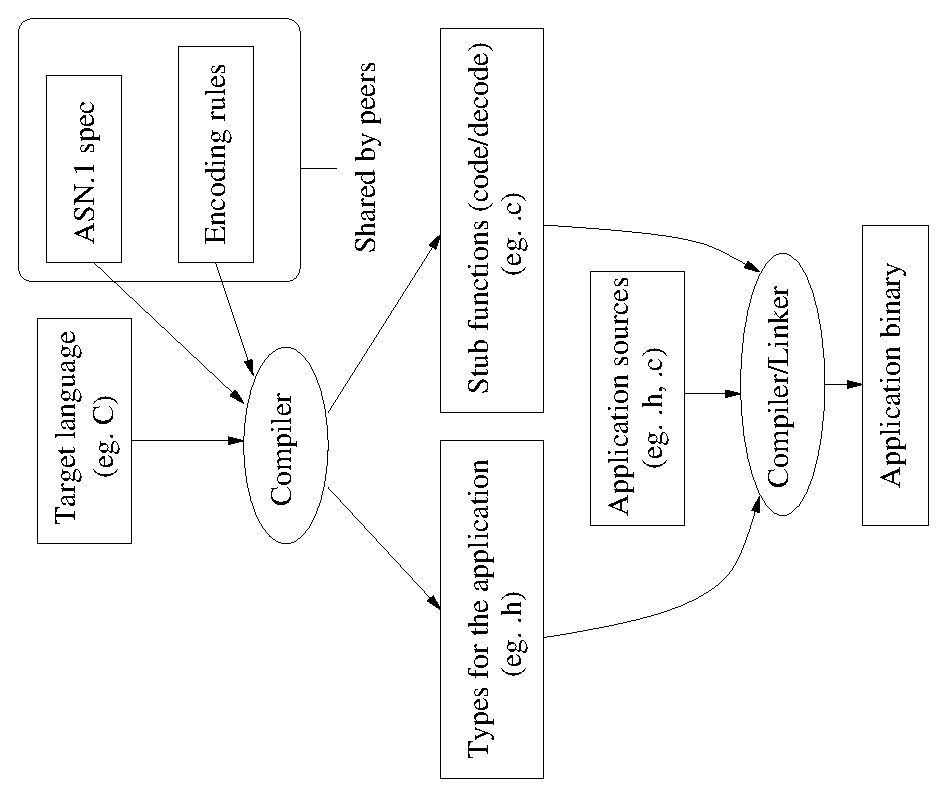
\includegraphics[scale=0.5]{compilation.eps}
\end{center}

\end{frame}

\begin{frame}
\frametitle{How do \ASN and the BER interact?}

\begin{itemize}

  \item Both peers share a common \ASN specification and agree upon
    the usage of the BER;

  \item each peer compile the \ASN specification to a set of type
    declarations and a set of coders/decoders (codecs) for each type;

  \item the target language may be different depending on the peer;

  \item the coders transform a value into a stream of bits according
    to the BER,

  \item the decoders transform a stream of bits into a value according
    to the BER (or reject it as ill-formed);

  \item these pieces of source code are compiled and linked separately
    against the corresponding communicating applications.

\end{itemize}

\end{frame}

\begin{frame}
\frametitle{General issues}

\begin{enumerate}

  \item Specifications: huge (704 pages A4 10pt), complex (concepts
  mutually dependent).

  \item Syntax: large and ambiguous grammar, dynamic extensions.

  \item English cannot tell the meaning of all combinations of
    syntactical constructs.

  \item Types denote value sets and type operators denote set
    operations: subtypes yield general set constraints.

  \item Encoding only applies to a subset of \ASN, defined
    implicitly and dependent on the encoding rules.

  \item Decoding is unspecified.

  \item Dynamic checks in codecs (depending on the target programming
    language) are unspecified.

  \item Open source or free compilers: extremely rare, unmaintaned,
    fragile, without precise error reporting.

\end{enumerate}

\end{frame}

%%%%%%%%%%%%%%%%%%%

\begin{frame}
\frametitle{Syntax analysis}

The BNF of \ASN spans 23~pages, versus 19~pages for ISO \Cpp.

\bigskip

When fed to Yacc as it is specified in the standards, it yields
between 3,000 and 4,000 shift/reduce and reduce/reduce conflicts
(for each kind!). It is ambiguous too.

\bigskip

The situation is actually much worse: many \emph{tokens} are
ambiguous, so if the lexer works without any extra knowledge from the
parser, there are even more conflicts.

\bigskip

I first solved the problem of the syntax analysis on the 1990
standard, which is smaller, albeit very nasty as well.

\end{frame}

%%%%%%%%%%%%%%%%%%%

\begin{frame}
\frametitle{Syntax analysis of \ASN 1990}

Too often engineers expect an off-the-shelf tool that will solve
parsing problems. If Yacc is put to work,
\begin{itemize}

\item it may not be suited for precise error reporting (bottom-up
  parsing, whilst more powerful than top-down, makes it more
  difficult to provide syntactical context for error reporting)

\item and understanding conflicts is done on the automaton, hence
  obscuring the relationship between the conflicts and the grammar
  (the parsing algorithm must be clearly held in mind at all times,
  because a conflict may involve several productions and a
  modification in one of them will change the automaton).

\end{itemize}

\bigskip

Real ingenuity and fortitude is needed, and I met an engineer who quit
after working six months on the syntax of \ASN (the company gave up
and is still paying an expensive license for a frontend).

\end{frame}

%%%%%%%%%%%%%%%%%%%

\begin{frame}
\frametitle{Syntax analysis of \ASN 1990 (cont.)}

Nevertheless, I devised a method and tools that help. It took me three
months to obtain an LL(1) grammar of \ASN and the corresponding
recursive descent parser, which was mathematically proved correct and
complete with respect to the standard BNF, and which reported syntax
errors very accurately.

\bigskip

Beyond the academic world, it was employed by some private
companies. The case I know best is that of the (ex) Southwestern Bell,
where they wanted to check the validity of their \ASN database, used
by all the subsidiaries of the group to define their telecommunication
protocols.

\end{frame}

%%%%%%%%%%%%%%%%%%%

\begin{frame}
\frametitle{Syntax analysis of \ASN 1990 (cont.)}

The programming language used to implement the parser was OCaml, but
the open source project Cryptix used the underlying, LL(1) grammar to
reimplement my parser in Java. See

\medskip

{\small\url{http://cryptix-asn1.sourceforge.net/ASN1-004.grammar}}

\medskip

Cryptix is an early library (still in use) for programming
cryptography in Java. (Check the ChangeLog file and search for errors
related to ``parsing''.)

\end{frame}

\begin{frame}[containsverbatim]
\frametitle{Incredibly short presentation of \ASN}

\noindent
\textbf{Primitive types}
\begin{itemize}

  \item \verb+ok BOOLEAN ::= TRUE+

  \item The \texttt{NULL} type has only one value, also noted
        \texttt{NULL};

\begin{verbatim}
zero INTEGER ::= 0
DayInTheYear ::= INTEGER {first(1), last(356)}
newYearsEve DayInTheYear ::= last
\end{verbatim}

  \item
\begin{verbatim}
SynchroIndicator ::= ENUMERATED {serial,parallel}
synchro SynchroIndicator ::= serial
\end{verbatim}

  \item

\begin{verbatim}
pi REAL ::= 3.14159
micron REAL ::= {mantissa 1,base 10,exponent -6}
\end{verbatim}

\end{itemize}

\end{frame}

\begin{frame}[containsverbatim]
\frametitle{More primitive types}

\begin{itemize}

  \item
\begin{verbatim}
byte BIT STRING ::= 'OD'H  -- or '00001110'B
T ::= BIT STRING {msb(7), lsb(0)}
v T ::= {msb, lsb}  -- or '10000001'B
\end{verbatim}

 \item The \texttt{OCTET STRING} type is similar to the \texttt{BIT
       STRING} for eight-bit multiples strings.

 \item The \texttt{OBJECT IDENTIFIER} and \texttt{RELATIVE-OID} types
       aim at referencing other \ASN modules (a set of type
       and value declarations) at an international level, by means of
       a path in a standard tree.

  \item For historical reasons, there are many string types.

\end{itemize}

\end{frame}

\begin{frame}[containsverbatim]
\frametitle{Some constructed types}

The \texttt{SET} type corresponds to the record-like structures in
programming languages:
\begin{verbatim}
PersonInfo ::= SET {age INTEGER, married BOOLEAN}
i PersonInfo ::= {married TRUE, age 46}
\end{verbatim}
Some fields can be marked as optional or having a default value:
\begin{verbatim}
Point ::= SET {x REAL DEFAULT 0, y REAL DEFAULT 0}
origin Point ::= {}           -- or {x 0.0, y 0.0}
\end{verbatim}

\end{frame}

\begin{frame}[containsverbatim]
\frametitle{Some constructed types (cont.)}

A real example:
\begin{verbatim}
DataAcknowledgementTPDU ::= SET {
  destRef        Reference,
  yr-tu-nr       TPDUnumber,
  checkSum       CheckSum OPTIONAL,
  subSeqNr       SubSequenceNumber DEFAULT 0,
  flowControlCnf FlowControlConfirmation OPTIONAL}
\end{verbatim}

The \texttt{SET OF} type corresponds to the mathematical notion of
sets with repetition:
\begin{verbatim}
T ::= SET OF INTEGER
empty T ::= {}
small T ::= {7, 9, 1, 1, 3}
\end{verbatim}

\end{frame}

\begin{frame}[containsverbatim]
\frametitle{Some constructed types (cont.)}

The \texttt{CHOICE} type corresponds to a \textbf{union} in C.
\begin{verbatim}
T ::= CHOICE {x REAL, y BOOLEAN}
u T ::= x : 0.5
v T ::= y : FALSE
\end{verbatim}
The Protocol Data Units (PDU) are \texttt{CHOICE} types, because they
model all the possible queries and responses between two peers. A
\texttt{CHOICE} type may be recursive, like the other constructed
types. One real example (a Network Management Protocol) is:
\begin{verbatim}
CMISFilter ::= CHOICE {
  item  FilterItem,
  and   SET OF CMISFilter,
  or    SET OF CMISFilter,
  not   CMISFilter}
\end{verbatim}

\end{frame}

\begin{frame}[containsverbatim]
\frametitle{Some subtyping constraints}

\ASN offers a very involved subtyping paradigm consisting of
constraints upon recursive types, that restricts their corresponding
sets of values in a set-theoritic manner, but also in a structural
way.
\begin{itemize}

  \item \textbf{Interval Constraint}: the \texttt{INTEGER},
  \texttt{REAL} and (almost all) string types have totally ordered
  values, hence allowing interval definitions. For instance:

\begin{verbatim}
PositiveOrZeroInteger ::= INTEGER (0..MAX)
PositiveInteger ::= INTEGER (0<..MAX)
NegativeOrZeroInteger ::= INTEGER (MIN..0)
NegativeInteger ::= INTEGER (MIN..<0)
PositiveReal ::= REAL (0<..PLUS-INFINITY)
NegativeReal ::= REAL (MINUS-INFINITY..<0)
RealInterval ::= REAL (4e-5..1e-4)
\end{verbatim}
\end{itemize}

\end{frame}

\begin{frame}[containsverbatim]
\frametitle{Some subtyping constraints (cont.)}

\begin{itemize}

  \item \textbf{Value Constraint}: to restrict the set of values of a
  type to be a singleton:

\begin{verbatim}
Wednesday ::= Day (wednesday)
\end{verbatim}

  \item \textbf{Union Constraint}: the new subtype contains the values
  of the first subtype and of the second subtype (keyword
  \texttt{UNION} or symbol ``\texttt{|}''):

\begin{verbatim}
Day ::= ENUMERATED {monday, tuesday, wednesday,
              thursday, friday, saturday, sunday}
WeekEnd ::= Day (saturday | sunday)
\end{verbatim}

  \item \textbf{Alphabet Constraint}: the strings can be restricted to
  be built upon a given alphabet:

\begin{verbatim}
CapitalAndSmall ::=
  IA5String (FROM ("A".."Z" | "a".."z"))
CapitalOrSmall ::= 
  IA5STring (FROM ("A".."Z") | FROM ("a".."z"))
\end{verbatim}

\end{itemize}

\end{frame}

\begin{frame}[containsverbatim]
\frametitle{Some subtyping constraints (cont.)}

\begin{itemize}

  \item \textbf{Size Constraint}: the values of string types may be
        constrained to a given sizes, introducing a constraint by the
        keyword \texttt{SIZE}:

\begin{verbatim}
Exactly31BitsString ::= BIT STRING (SIZE (31))
StringOf31BitsAtTheMost ::=
  BIT STRING (SIZE (0..31))
NonEmptyString ::= BIT STRING (SIZE (1..MAX))
\end{verbatim}

The size constraint can also apply to \texttt{SET OF} types. In that
case, the semantics is very different: the values of the types are
sets whose \emph{cardinals} are specified by the size constraint:

\begin{verbatim}
SetOf5Strings ::=
  SET (SIZE(5)) OF PrintableString
SetOfStringsOf5Char::=
  SET OF PrintableString (SIZE(5))
\end{verbatim}

\end{itemize}

\end{frame}

\begin{frame}[containsverbatim]
\frametitle{Some subtyping constraints (cont.)}

\begin{itemize}

  \item \textbf{Intersection Constraint}: the new subtype contains the
        values that belong to the two subtypes (keyword
        \texttt{INTERSECTION} or symbol \texttt{\symbol{94}}):

\begin{verbatim}
FrenchPhoneNumber ::= 
  NumericString (FROM ("0".."9") ^ SIZE (10))
\end{verbatim}

  \item \textbf{Inclusion Constraint}: to restrict a subtype to have
        only the values of a given subtype (optional keyword
        \texttt{INCLUDES}):

\begin{verbatim}
LongWeekEnd ::=
  Day ((INCLUDES (WeekEnd)) | monday)
Bis ::= Day (WeekEnd | monday)
\end{verbatim}
\end{itemize}

\end{frame}

\begin{frame}[containsverbatim]
\frametitle{Some subtyping constraints (cont.)}

\begin{itemize}

  \item \textbf{Complement Constraint}: to restrict the values of a
        type to \emph{not} belong to another subtype:

\begin{verbatim}
Lipogramme ::=
  IA5String (FROM (ALL EXCEPT ("e" | "E")))
\end{verbatim}

\bigskip\bigskip

  \item \textbf{Constraint on \texttt{SET OF}}: to restrict the
        elements of a \texttt{SET OF} value:

\begin{verbatim}
TextBlock ::= SET OF VisibleString
AddressBlock ::=
  TextBlock (WITH COMPONENT (SIZE(1..32)))
\end{verbatim}

\end{itemize}

\end{frame}

\begin{frame}[containsverbatim]
\frametitle{Some subtyping constraints (cont.)}

\begin{itemize}
  \item \textsf{Partial Constraint}: to restrict \emph{some} fields
        of a \texttt{SET} or \texttt{CHOICE}:

\begin{verbatim}
Quadruple ::= SET {
  alpha ENUMERATED {in, out} OPTIONAL,
  beta  IA5String OPTIONAL,
  gamma SET OF INTEGER,
  delta BOOLEAN DEFAULT TRUE}
\end{verbatim}

we can derive a subtype whose component \verb+alpha+ is always present
and equals \verb+in+, and the component \verb+gamma+ always has
five elements:
\begin{verbatim}
Quadruple1 ::=
  Quadruple (WITH COMPONENTS {..., 
                              alpha (in) PRESENT,  
                              gamma (SIZE (5))})
\end{verbatim}

\end{itemize}

\end{frame}

\begin{frame}[containsverbatim]
\frametitle{Some subtyping constraints (cont.)}

This subtype has the same values as:
\begin{verbatim}
Quadruple1 ::= SET {
  alpha ENUMERATED {in, out} (in),
  beta  IA5String OPTIONAL,
  gamma SET SIZE (5) OF INTEGER,
  delta BOOLEAN DEFAULT TRUE}
\end{verbatim}

\end{frame}

\begin{frame}[containsverbatim]
\frametitle{Practical issues in validation}

\ASN types are considered as sets of values, thus types must have at
least one (finite) value.

\bigskip

Because of the great expressivity of \ASN, the compilers are not
likely to fully check arbitrary combinations of subtyping
constraints:
\begin{itemize}

   \item an incorrect specification is badly rejected: \\
         \verb+T ::= T+ \ \ produces \ \ \verb+typedef T T;+ \\ 
         before being rejected by a C~compiler;

   \item a correction specification is rejected:
\begin{verbatim}
T ::= SET (WITH COMPONENT (0)
          | WITH COMPONENT (1)) OF INTEGER
\end{verbatim}

           \item an incorrect specification is accepted:\\
                 \verb+a INTEGER (0<..9) ::= 0+
\end{itemize}

\end{frame}

\begin{frame}[containsverbatim]
\frametitle{Incompleteness of the standard}

\begin{itemize}

  \item Aliasing\\
        \texttt{a T1 ::= <\emph{a value of type} T1>}\\
        \texttt{b T2 ::= a} \\
        What conditions on \texttt{T1} and \texttt{T2}?

  \item Recursive types and values:
\begin{verbatim}
T ::= SET OF T
x T ::= {x}
y T ::= {{}}
\end{verbatim}

\end{itemize}

\end{frame}

\begin{frame}
\frametitle{Theoretical Problems}

\begin{enumerate}
  
  \item \label{finiteness} the types may have only infinite
        values:\\
        \texttt{T ::= SET \{a T\}};

  \item \label{type_conformance} some value declarations may be
        ill-typed:\\
        \texttt{v REAL ::= ""};

  \item \label{type_compatibility} especially, some value references
        may be ill-typed, as\\
        \texttt{a VisibleString ::= b}\\
        \texttt{b INTEGER ::= 0};

  \item \label{constraint_consistence} the subtype constraints may
        be inconsistent:\\
        \texttt{T ::= REAL (SIZE(7))};

  \item \label{subtype_non_emptiness} the subtypes may be empty, as\\
        \texttt{T ::= SET ((SIZE (1)) \symbol{94} (SIZE (2))) OF REAL};
        
  \item \label{solvability} the subtypes may have no value set:\\
        \texttt{T ::= REAL (ALL EXCEPT T)}. 

\end{enumerate}

\end{frame}

\begin{frame}
\frametitle{Problems (cont.)}

In other words, the issues to settle are respectively:
\begin{enumerate}

  \item the finiteness problem;
 
  \item the typechecking problem;

  \item the type compatibility problem;

  \item the constraint consistence problem;

  \item the non-emptiness problem;

  \item the solvability problem.

\end{enumerate}

\end{frame}

\begin{frame}
\frametitle{Analysis}

\begin{itemize}

  \item type compatibility $\subseteq$ typechecking;

  \item constraint consistence, non-emptiness $\subseteq$ solvability
        (the system is solved when we construct explicitly the values
        of each subtype);

  \item typechecking $\subseteq$ solvability:
\begin{tabular}{@{}r@{\,}c@{\,}l@{}}
   \texttt{y INTEGER (0..9) ::= 1}
   & $\rightarrow$ 
   & $\left\{
       \begin{tabular}{@{\,}l@{}} 
           \texttt{y A ::= 1} \\
           \texttt{A ::= INTEGER (0..9)} \\
           \texttt{B ::= A (y)}
        \end{tabular}
     \right.$
\end{tabular}
where \texttt{A}~and~\texttt{B} are fresh type references.

\end{itemize}

So, finiteness and solvability are enough to get a full validation of
\ASN.

\end{frame}

\begin{frame}
\frametitle{Two approaches for validation}

Every \ASN specification is rewritten in a subset of same
expressiveness, with less syntactical constructs. Two strategies:
\begin{enumerate}

  \item Few preliminary rewrites, followed by a collection of set
  constraints, then fed to a generic constraint solver.

  \item Lots of preliminary rewrites, simple algorithms to check
    solvability. (This is like taking the previous method and
    interleave a dedicated solver with the syntactical rewrites.)

\end{enumerate}
Comparison:
\begin{enumerate}

\item Pros: modularity, less programming. Cons: constraints too
  general for off-the-shelf solvers.

  \item Pros: easy checking. Cons: heavily specialised, correctness
    hard to assess.

\end{enumerate}
We need to find a trade-off.

\end{frame}

\begin{frame}
\frametitle{Set Constraints}

Sets constraints are inclusions between expressions interpreted over
the domain of sets of trees which may be recursively defined.

\medskip

The \ASN types, by having a tree structure (technically, they are
rational trees), fit perfectly in the usual domain of set
constraints.

\medskip


A set constraint has the form $\alpha \subseteq \beta$, where $\alpha$
and $\beta$ are \emph{set expressions}. Examples are \textsf{0} (the
empty set), \textsf{1} (the set of all terms), $\alpha$ (a set-valued
variable), $c(\alpha, \beta)$ (a constructor application), and the
union, intersection or complement of set expressions. Given a set of
constructors ${\cal C}$, where each $c \in \mathcal{C}$ has arity
$a(c)$, set expressions are defined by the grammar:
\begin{equation*}
E ::= \textsf{0} \mid \textsf{1} \mid \alpha \mid c (E_1, \ldots,
E_{a(c)}) \mid E_1 \cup E_2 \mid E_1 \cap E_2 \mid \neg E_1.
\end{equation*}

\end{frame}

\begin{frame}
\frametitle{Common Application}

In general, set constraints are used in the static analysis of
programs: they are the smallest supersets of the sets of the computed
values. Solving these constraints means constructing these
approximated sets (\emph{e.g.}, for optimisation).

\medskip

For example, consider a program with two uses of a variable
$v$. Assume that from one use we determine that $v$ must be a number
(\emph{i.e.}, $v \subseteq \textsf{Int} \, \cup \, \textsf{Float}$)
and from the other use that $v$ cannot be an integer (\emph{i.e.}, $v
\subseteq \neg\textsf{Int}$). Combining these constraints, we can
infer that $v$ must be a floating point number (\emph{i.e.}, $v
\subseteq (\textsf{Int} \, \cup \, \textsf{Float}) \cap
\neg\textsf{Int} = \textsf{Float}$).

\end{frame}

\begin{frame}
\frametitle{Application to \ASN}

In order to apply the set constraints to \ASN we define specific
constructors that model all the subtyping constraints (like parsing to
obtain an abstract syntax tree).

\medskip

Then, the problem consists in extracting set constraints from each
subtype, such as their solving provide a mapping from the subtype to
its set of values: this is a kind of \emph{denotational semantics} of
\ASN.

\medskip

As far as validation is concerned, if some constraints are unsolvable
or the set of solutions is empty, them the specification must be
rejected.

\medskip

Aiken and Wimmers (1993) proposed the first solving algorithm for the
class of constraints we are using, \emph{but there are practical
  limitations.}

\end{frame}

\begin{frame}
\frametitle{What are the Basic Encoding Rules (BER)?}

\begin{itemize}

  \item The BER are a set of rules defining the serialisation into
    bits of \ASN values;

  \item the bit frames (\emph{codes} or \emph{encodings}) have a
    uniform structure: a triple made of a \emph{tag}, a \emph{length}
    and some \emph{contents};

  \item the tag field is extracted from the data type,

  \item the contents field is extracted from the data itself,

  \item the length field is computed over the contents field,

  \item the structure allows embedding of sub-frames (in the contents
    field)

  \item and an \emph{indefinite length} form, as a sender's option.

\end{itemize}
\end{frame}

\begin{frame}
\frametitle{So, what is wrong with the BER?}

Some years ago, the press reported several alleged vulnerabilities
relating \ASN and the BER to SNMP and OpenSSL, about improper decoding
(and rejection) of ill-formed BER encodings leading to
\begin{itemize}
  \item buffer overflows,

  \item unspecified (non-deterministic) behaviours,

  \item stack corruptions,

  \item hence possible denials of service.

\end{itemize}

I showed that the joint design of \ASN and the BER is sound, and that
the problems lay with the back-ends of the compilers.

\end{frame}

\begin{frame}
\frametitle{Advantages of formalisation}

\begin{enumerate}

  \item For the standardisation committees:
    \begin{itemize}

    \item Help find incompletenesses, ambiguities, inconsistencies and
      unneeded restrictions;

    \item If an encoding is also formalised, proofs of desirable
      properties, like correctness, become possible.

    \end{itemize}

  \item For the tool makers:
    \begin{itemize}

      \item If expressed declaratively, the formalisation can also
        define abstract algorithms for the front-end of an \ASN
        compiler.

    \end{itemize}

\end{enumerate}

\end{frame}

\begin{frame}
\frametitle{Modelling (assumptions and encoding)}

We start making some assumptions that abstract away low-level details
and help us capturing the design principles of the BER:
\begin{itemize}

  \item values are given in \ASN, not in the application language (in
  fact they are produced in memory at run-time);

  \item codes are tuples, not bit series, in order to easily reason by
  induction on their structure;

  \item the network is reliable (no alteration of codes).

\end{itemize}
BER codes may not be unique for a given value, due to possible
sender's options (\emph{e.g.}, encoding of booleans or unordered
sets).
\begin{proposition}
All the BER encodings of a given value, according to a given type, are
equivalent.
\end{proposition}

\end{frame}

\begin{frame}
\frametitle{Modelling (decoding)}

\begin{itemize}

  \item The BER standard (26~pages of English) does not define the
  decoding at all.

  \item We believe that the receiver is the peer most concerned with
  the sound design of the BER: \emph{the composition of encoding and
  decoding yields a value equivalent to the original one}.

  Hence we need an equivalence relationship between values
  (thus independent from the BER).

\end{itemize}

  \begin{theorem}[Soundness]
    Let $v$ be a value of type $T$. Then the BER decoding of
    \emph{any} BER encoding of $v$ is equivalent to $v$.
  \end{theorem}

\end{frame}

\begin{frame}
\frametitle{Soundness property}

\centerline{\includegraphics[width=.85 \textwidth]{model-1.eps}}

\end{frame}


\begin{frame}
\frametitle{Equivalence entailment}

As a consequence, in order to prove the soundness property, it appears
that we need to link logically the two equivalence relationships we
defined separately on codes and values.

\begin{proposition}[Equivalence entailment]
Let $c_1$ and $c_2$ be two equivalent codes. Then the decoding of
$c_1$ is equivalent to the decoding of $c_2$ assuming the same type.
\end{proposition}

\bigskip

One equivalence relies solely on the BER and the other one is inherent
to \ASN. Hence \emph{this proposition is the link between the design
  of \ASN and the design of the BER}.

\end{frame}

\begin{frame}
\frametitle{Core \ASN}

\begin{itemize}

  \item The BER only apply to a subset \ASN (whose definition spans 
  188~pages).

  \item This suggests that the whole \ASN can be reduced to an inner
  subset which has the same expressivity, we call \emph{BER domain}.

  \item In fact it is even possible to reduce further the BER domain
  to a smaller subset, we call \emph{\core}, in which formal
  reasoning is easier.

  \item The formal definition of these reductions is achieved by means
  of a series of rewriting rules that preserve the set of values of
  the specifications (or of a given type).

  \item We can easily check some useful properties in \core:
  \begin{theorem}[BER termination]
    The encoding of \core values with the BER always terminates.
  \end{theorem}

\end{itemize}

\end{frame}

\begin{frame}
\frametitle{Core \ASN and soundness property}

\centerline{\includegraphics[width=.85 \textwidth]{model-2.eps}}

\end{frame}

\begin{frame}
\frametitle{Back to our model}

\begin{itemize}

  \item Let us note $\coding{\Gamma}{v}{T}{c}$ the judgement ``In the
    environment $\Gamma$, the value $v$ is encoded into the code $c$,
    following the type $T$.''  (The environment models the \ASN
    module.)

  \item Let us note $\decoding{\Gamma}{c}{T}$ the decoding of $c$ in
    the environment $\Gamma$ according to type $T$.

  \item We already noted $v_1 \approx v_2$ the equivalence of values
    $v_1$ and $v_2$

  \item and $c_1 \sim c_2$ the equivalence of codes $c_1$ and $c_2$.

\end{itemize}

The next step consists in defining these relations by means of systems
of inference rules.

\end{frame}

\begin{frame}
\frametitle{Formal model}

We can now rephrase formally our propositions:
\begin{itemize}

  \item Proposition ``All the BER encodings of a given value,
  according to a given type, are equivalent.'' becomes

  \begin{proposition}
    If $\coding{\Gamma}{v}{T}{c_1}$ and $\coding{\Gamma}{v}{T}{c_2}$
    then $c_1 \sim c_2$.
  \end{proposition}

  \item Proposition ``The decoding of two equivalent codes lead to two
  equivalent values.'' becomes

  \begin{proposition}[Equivalence entailment]
    $c_1 \sim c_2 \Longrightarrow \decoding{\Gamma}{c_1}{T} \approx
    \decoding{\Gamma}{c_2}{T}$
  \end{proposition}

  \item Theorem ``Let $v$ be a value of type $T$. Then the BER
    decoding of \emph{any} BER encoding of $v$ is equivalent to $v$.''
    becomes

  \begin{theorem}[Soundness]
    If $\coding{\Gamma}{v}{T}{c}$ then $\decoding{\Gamma}{c}{T}
    \approx v$.
  \end{theorem}

\end{itemize}

\end{frame}

\begin{frame}
\frametitle{Model-based testing}

During my doctoral studies, I only considered the transmission of
data. When I started as a research engineer, I got to work on the
control part of communication protocols, and the generation of test
suites for their implementation, derived from their specification.

\bigskip

This work (1998) is still quoted in research papers nowadays (this
month, actually).

\end{frame}

\begin{frame}
  \frametitle{Didactics of programming}

  During my decade as a professor, I got interested in the didactics
  of programming, the mental models of students, the teaching
  methodoly, and the relationship with programming language design.

  \bigskip

  I published a book entitled \emph{Design and Analysis of Purely
    Functional Programs} (650 pages) and several papers in the field
  of didactics of informatics.

  \bigskip

  You can download my book and papers at
  \begin{center}
  \url{http://crinderknecht.free.fr/CV/index.html}
  \end{center}
  
  \bigskip

  This is also a work that is quoted nowadays.

\end{frame}

\begin{frame}
  \frametitle{Pet projects}

  \begin{itemize}

    \item I translate poetry from Spanish to French and vice versa. I
      published in 1998 the only translation in French of Pablo
      Neruda's \emph{Twenty Love poems and a Desperate Song}. Sales
      are strong!

    \item I occasionally write poetry myself. (Unpublished.)

    \item For the last ten years, I have been working on a build
      system for OCaml, based on GNU~Make.

  \end{itemize}

\end{frame}

\end{document}
